%!TEX root = PhD_Thesis.tex
\chapter[Human-in-the-Loop Control]{Human-in-the-Loop Control of Pre-Clinical Needle Steering}

\section{Introduction}
The experimental results presented in Chapter 4 showed promising accuracy for autonomous targeting of the needle tip. While these tests were performed in biological tissues, they were completed in a bench-top setting, over a relatively small needle steering workspace. In this chapter we moved to a more realistic pre-clinical environment, using a porcine cadaver in a simulated interventional radiology suite. 

Moving to a more realistic test environment revealed several limitations of our bench-top techniques. The mechanical 3D ultrasound transducer has a limited field of view relative to the size of the liver, and any transducer motion invalidates existing data. In previous chapters, the transducer was clamped relative to the tissue. In this chapter, we use an electromagnetic tracking system to enable freehand 3D ultrasound. 

The appearance of the vibrating needle in Doppler ultrasound can be highly irregular in realistic imaging arrangements. While the Doppler approach still provides an indication of needle pose, much more sophisticated segmentation algorithms would be needed for the fully autonomous control approach described in Chapter 2 and Chapter 4. In this chapter, we use the Doppler technique to indicate the approximate needle pose to a human user, and allow the user to manually localize the needle tip. Also, our software implementations in Chapters 2 and 4 did not provide real-time visualization of 3D ultrasound data, needle pose, target location, etc. In this chapter, we implement a user interface that allows visualization and user control during steering. 

The remainder of this chapter is divided into three sections. Section~\ref{sec:HumanInTheLoopImplementation} describes the algorithmic, hardware, and software implementation of our human-in-the-loop approach to pre-clinical needle steering. Section~\ref{sec:HumanInTheLoopValidation} describes experimental validation of our method in bench-top and porcine-cadaver tests. Section~\ref{sec:HumanInTheLoopResults} presents and discusses the results. The work presented in this chapter was completed in collaboration with Dr. Gloria Hwang and Joseph Greer.

\section{Implementation}
\label{sec:HumanInTheLoopImplementation}

\subsection{Robot and Steerable Needles}
\label{sec:NS2RobotAndNeedle}
Chapter 3 presented a new articulated-tip steerable needle that showed promising curvature results in biological tissue. Unfortunately, as discussed in that chapter, the plastic construction of the miniature hinges failed too frequently to be used in a pre-clinical setting. (Chapter 6 discusses possible future improvements to the hinge design.) In this chapter, we applied the exaggerated tip geometry suggested by the results of Chapter 3, but used a flexure tip, consisting of a rectangular Nitinol wire plastically deformed to the desired tip angle. This tip is able to pass through an introducer sheath because of the large elastic range of Nitinol, but still returns to its bent shape inside tissue. A similar flexure tip was previously proposed by Swaney et al.~\cite{Swaney2013}. Their design used two sections of Nitinol tubes, with multiple Nitinol wires adhered between the sections to form a flexure. Fig.~\ref{fig:NS2AndNeedle} shows the flexure tip steerable needle, and the robot used to drive it in this chapter.

\begin{figure}[!t]
\centering
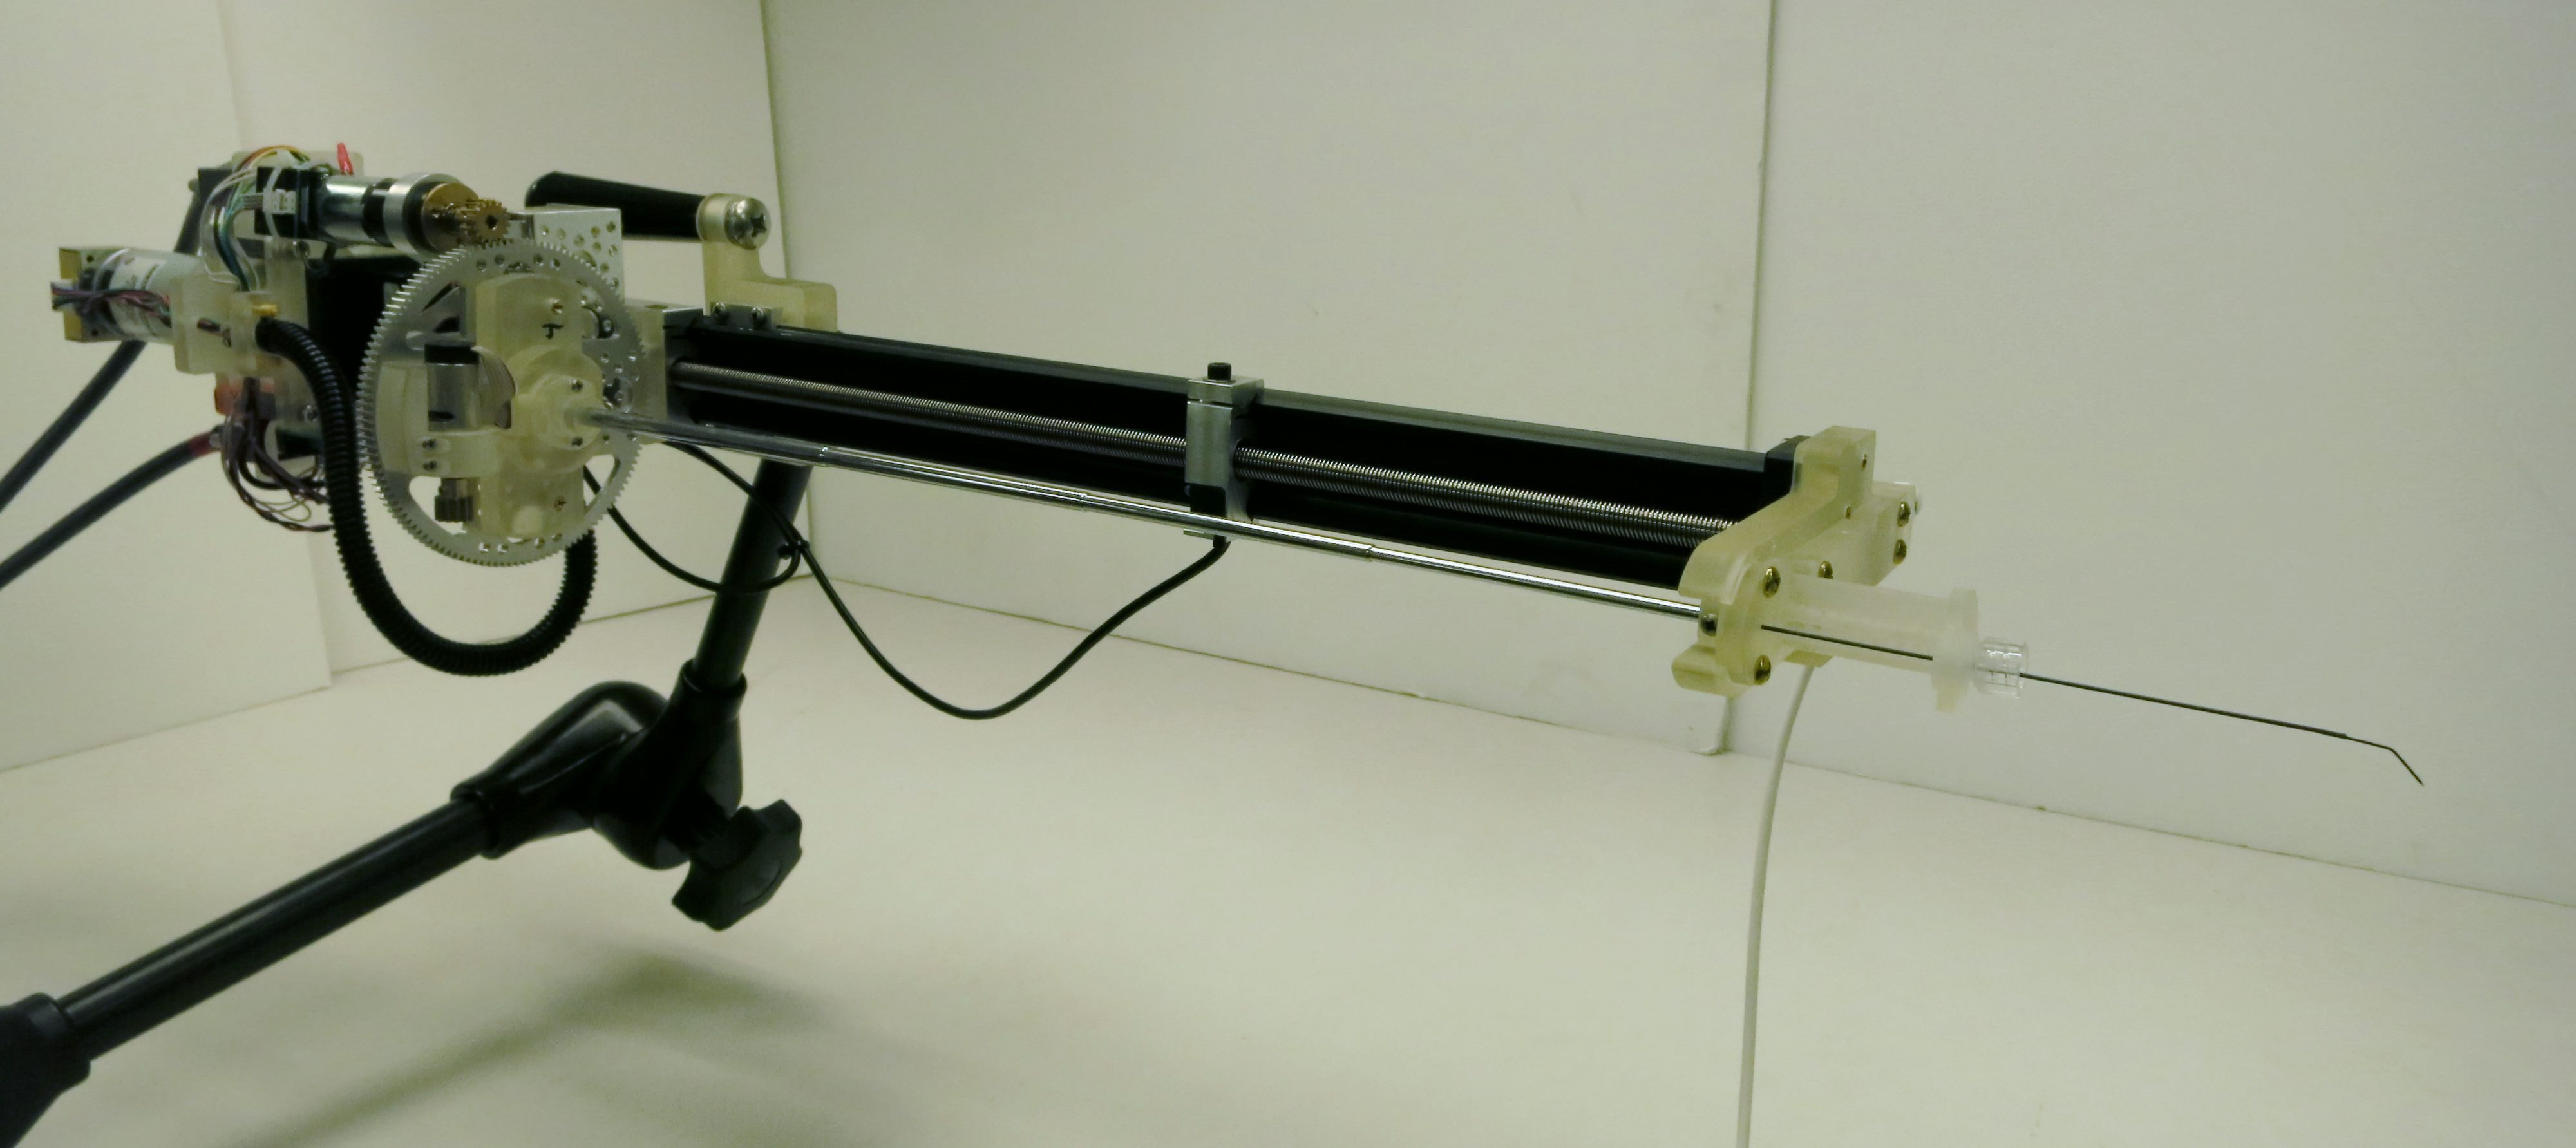
\includegraphics[width = \columnwidth]{./Images/Chapter5/NS2RobotAndNeedle/NS2RobotAndNeedle.jpg}%
\caption[Robot and flexure-tip steerable needles]{Portable needle steering robot with positioning arm and handle, flexure-tip steerable needle with integrated anti-buckling sheath and luer connector fitting for introducer needle.}
\label{fig:NS2AndNeedle}
\end{figure} 

\subsection{Control Modes}
Our implementation of human-in-the-loop control allows the user to select between joint-space control of the needle steering robot and task-space control of the needle tip position. In joint-space control, the user uses a 3D mouse (SpaceNavigator; 3Dconnexion, Boston, MA) to directly control the insertion and rotation of the needle steering robot's two DOF. Using a rate-control scheme, uniaxial displacement of the 3D mouse is mapped to insertion velocity, while uniaxial rotation of the 3D mouse is mapped to rotation speed. Fig.~\ref{fig:InputDevices} shows the 3D mouse.

\begin{figure}[!t]
\centering
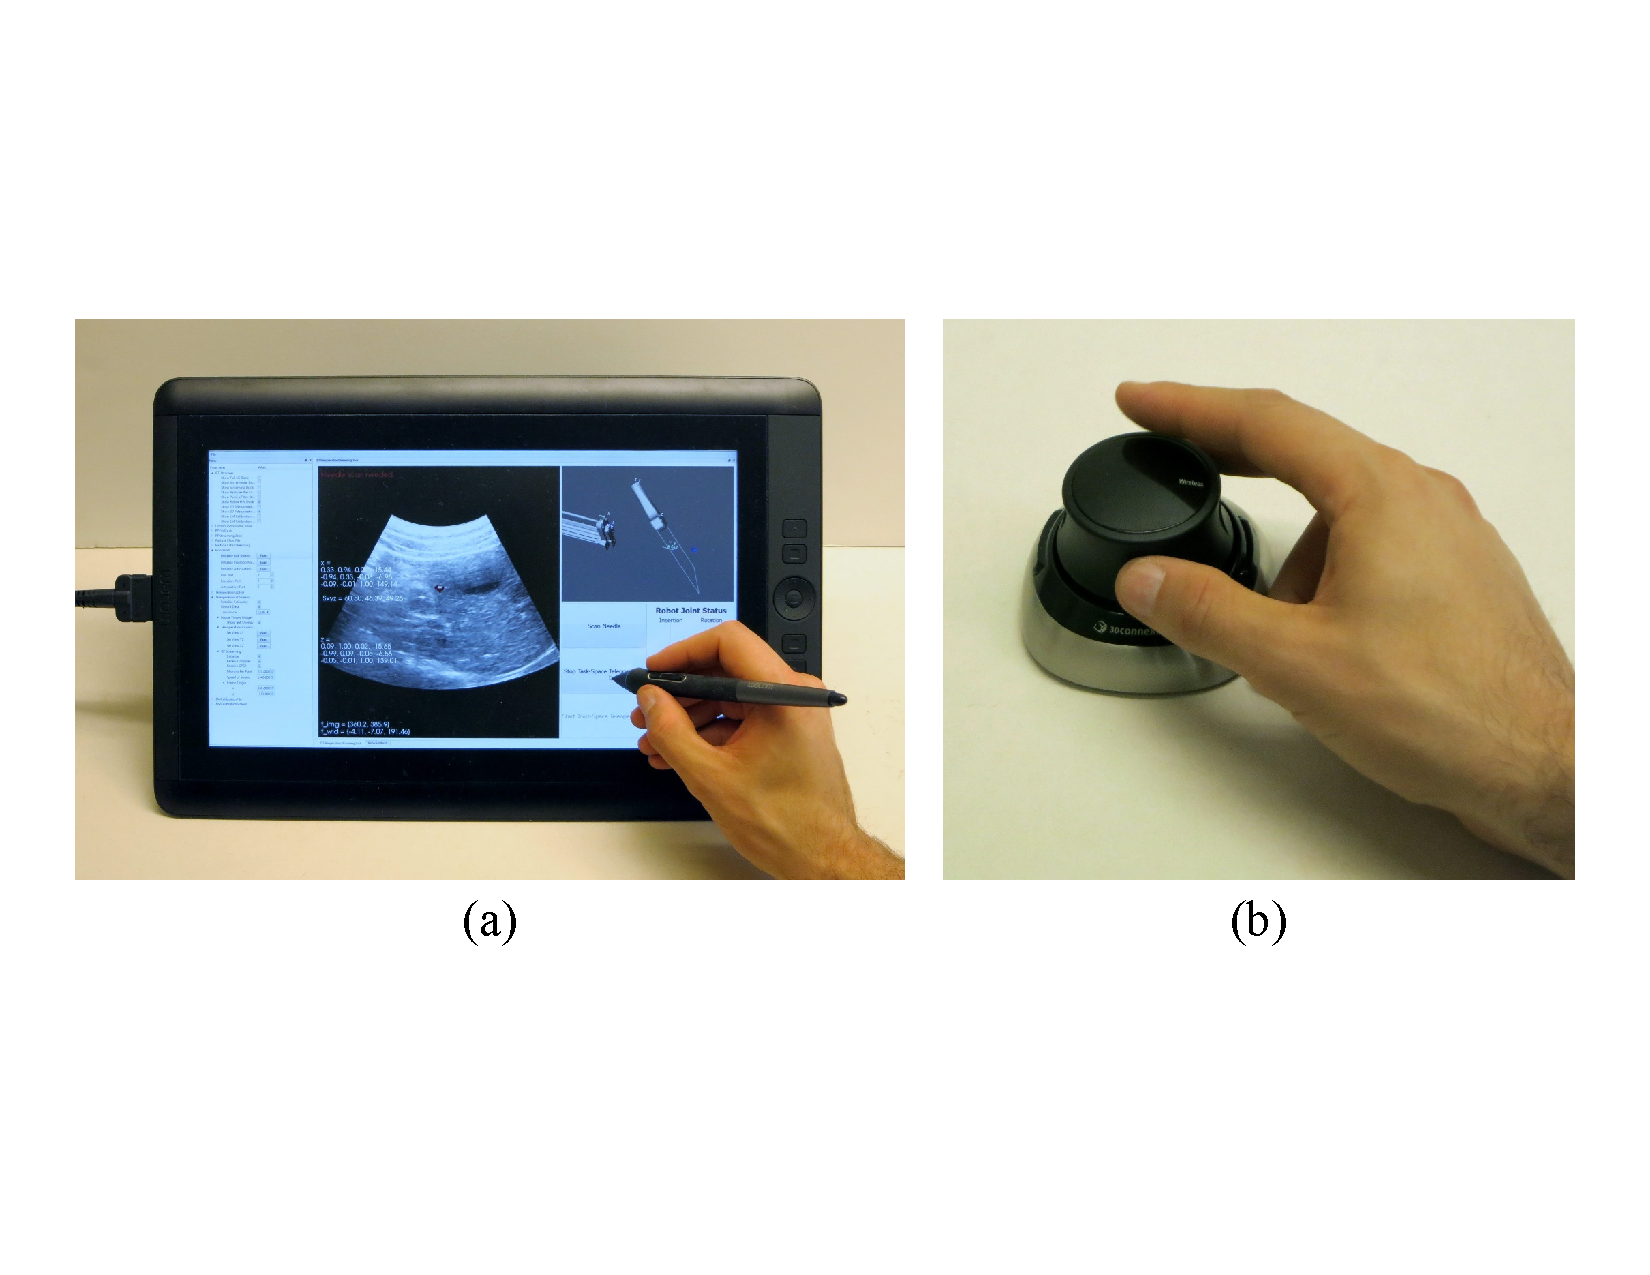
\includegraphics[width = \columnwidth]{./Images/Chapter5/InputDevices/InputDevices.pdf}%
\caption[Input devices for robot control]{Input devices for human-in-the-loop control: (a) A 3D mouse is used for rate control of the steerable needle insertion and rotation. (b) A tablet is used to select targets and the needle tip position in the stream of 2D ultrasound images.}
\label{fig:InputDevices}
\end{figure}  

In task-space control, the user selects the target position $t$ directly in the live 2D ultrasound image using a tablet interface (Cintiq 13; Wacom Co., Vancouver, WA). The tablet interface is shown in Fig.~\ref{fig:InputDevices}. The robot then steers the needle towards the target automatically, with feedback based on the output from the UKF estimation scheme described in Chapter 4. Fig~\ref{fig:ClinicalBlockDiagram} shows a block diagram of our closed-loop task-space control approach. The estimate is updated without measurement feedback (i.e., based on the process model) at the ultrasound machine's native framerate. After every 10~mm of insertion, the system requires a tip-position measurement, which the user provides by scanning over the needle tip with the ultrasound probe, and then localizing it using the tablet interface. The estimation scheme is implemented exactly as described in Chapter 4, with two exceptions. First, the process and measurement noise levels were again experimentally characterized for the flexure needle and manual measurements, and the filter gains were adjusted accordingly. Second, the manual measurements only provided feedback on tip position, so tip orientation feedback was set to the estimator output with extremely low gain (high variance). This approach avoided practical computational problems related to matrix inversion. 

In Chapter~2 and Chapter~4, closed-loop needle steering was achieved by using a steering controller to identify a desired path from each measured tip position to the target, and using open-loop duty-cycle control to follow the desired path. In this chapter, where the unscented Kalman filter was updated at a higher frequency (the ultrasound framerate), we used a sliding mode controller to avoid the need for explicit duty-cycle control. In sliding mode control of needle steering, which was proposed by Rucker et al.~\cite{Rucker2013}, the target position $t$ is projected onto the $x$-$y$ plane of the needle tip frame. The needle rotation is constantly adjusted by the minimum angle $\delta\theta$ so that the projected target point is aligned with the $y$ axis of the tip frame (the direction of curvature). Under ideal controller action, when the needle insertion velocity is slow relative to the rotation velocity and the target is within a reachable region, the needle tip's trajectory will converge to the target. This approach eliminates the need for explicit duty-cycle control~\cite{Minhas2007}. 

\begin{figure}[!t]
\centering
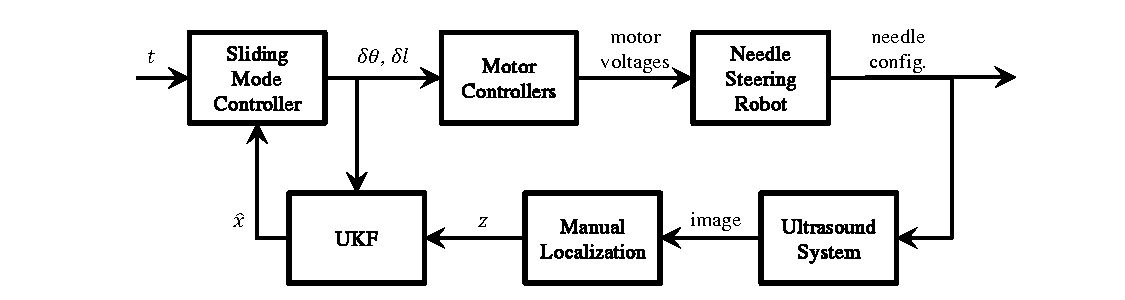
\includegraphics[width=\columnwidth]{Images/Chapter5/ClinicalBlockDiagram/ClinicalBlockDiagram}%
\caption[Block diagram of closed-loop task-space control algorithm]{Block diagram of closed-loop task-space control. Manual localization of the needle tip from freehand 3D ultrasound data provides a noisy measurement of needle tip pose to the UKF estimation scheme. The output of the estimation scheme is used as input by the sliding mode controller.}
\label{fig:ClinicalBlockDiagram}
\end{figure}

\subsection{Freehand 3D Doppler Ultrasound Imaging}
As in the previous chapters, a SonixMDP ultrasound console (Ultrasonix Medical Corp., Richmond, Canada) was used for imaging. Unlike in the previous chapters, a 2D curvilinear transducer (C5-2/60) with an integrated electromagnetic tracking element was used. Fig.~\ref{fig:freehand3DUS} depicts this arrangement. The calibrated electromagnetic tracking system, branded as SonixGPS by Ultrasonix, allows the 3D context of the 2D ultrasound image data to be resolved in real time. 

\begin{figure}[!ht]
\centering
\includegraphics[width = 0.9\columnwidth]{./Images/Chapter5/Freehand3DUS/Freehand3DUS.pdf}%
\caption[Freehand 3D ultrasound imaging arrangement]{Freehand 3D ultrasound imaging arrangement and relevant coordinate systems. The pose of the needle tip, defined by $\{p,R\}$, is measured using a 2D ultrasound transducer with integrated tracking element and pose defined by $\{p_{\text{US}},R_{\text{US}}\}$. The transducer is tracked relative to the electromagnetic base station with pose $\{p_{\text{EM}},R_{\text{EM}}\}$. The tracker information is referred to the robot frame $\{p_{\text{robot}},R_{\text{robot}}\}$ using a tracking element in the distal section of the robot, and a stylus calibration.}
\label{fig:freehand3DUS}
\end{figure}

\begin{figure}[!ht]
\centering
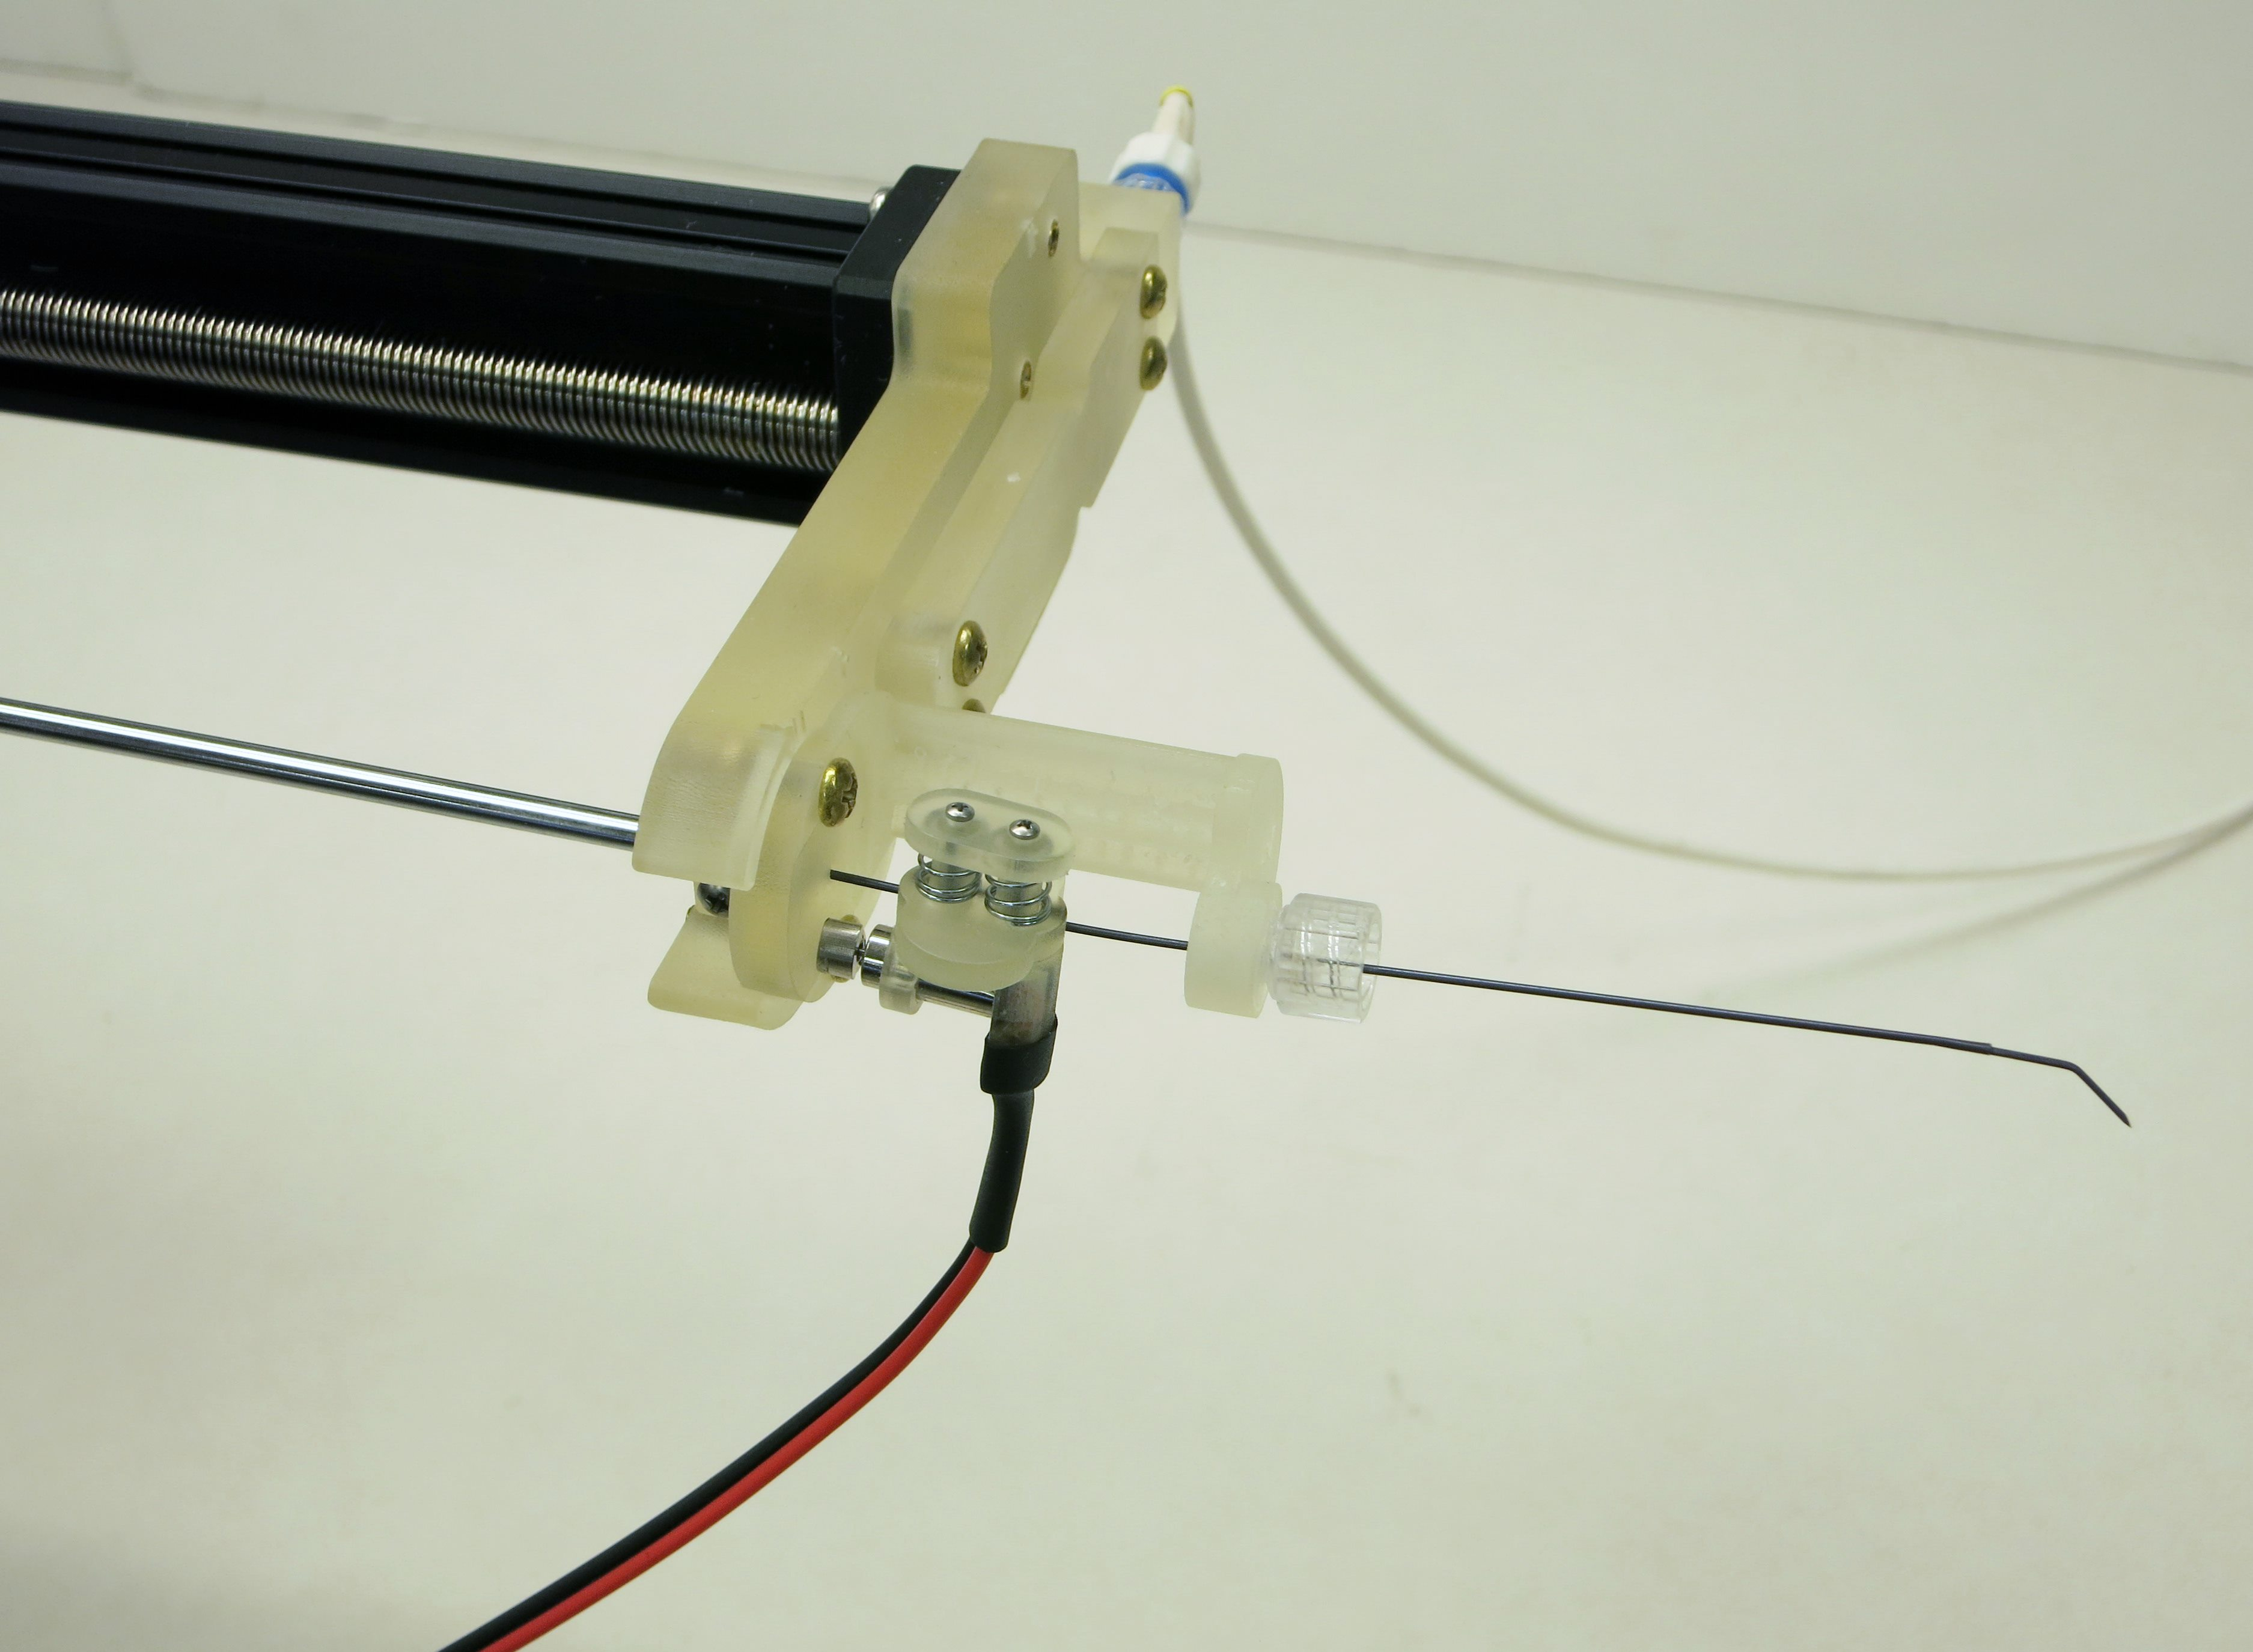
\includegraphics[width = 0.5\columnwidth]{./Images/Chapter5/Buzzer/Buzzer.jpg}%
\caption[Disposable vibration device]{Disposable vibration device for ultrasound Doppler imaging. A 3D-printed spring-loaded clip attaches a vibration motor to the steerable needle shaft. The unit is battery powered and entirely disposable. Motion along the needle shaft is constrained by an enclosure.}
\label{fig:Buzzer}
\end{figure}  

As in Chapter 2, external vibrations were applied to the proximal end of the steerable needle shaft. However, in this chapter, a spring-loaded clip was used to attach a vibration motor (a miniature DC motor spinning a small eccentric mass) to the steerable needle shaft. Fig.~\ref{fig:Buzzer} shows the new vibration device. Compared to the integrated piezoelectric vibration device described in Chapter 2, this system has the advantages that it is completely disposable if contaminated with bodily fluids, and it can be visually monitored during insertion and retraction to ensure good coupling. These characteristics were identified as necessary after early pre-clinical testing.

\begin{figure}[!t]
\centering
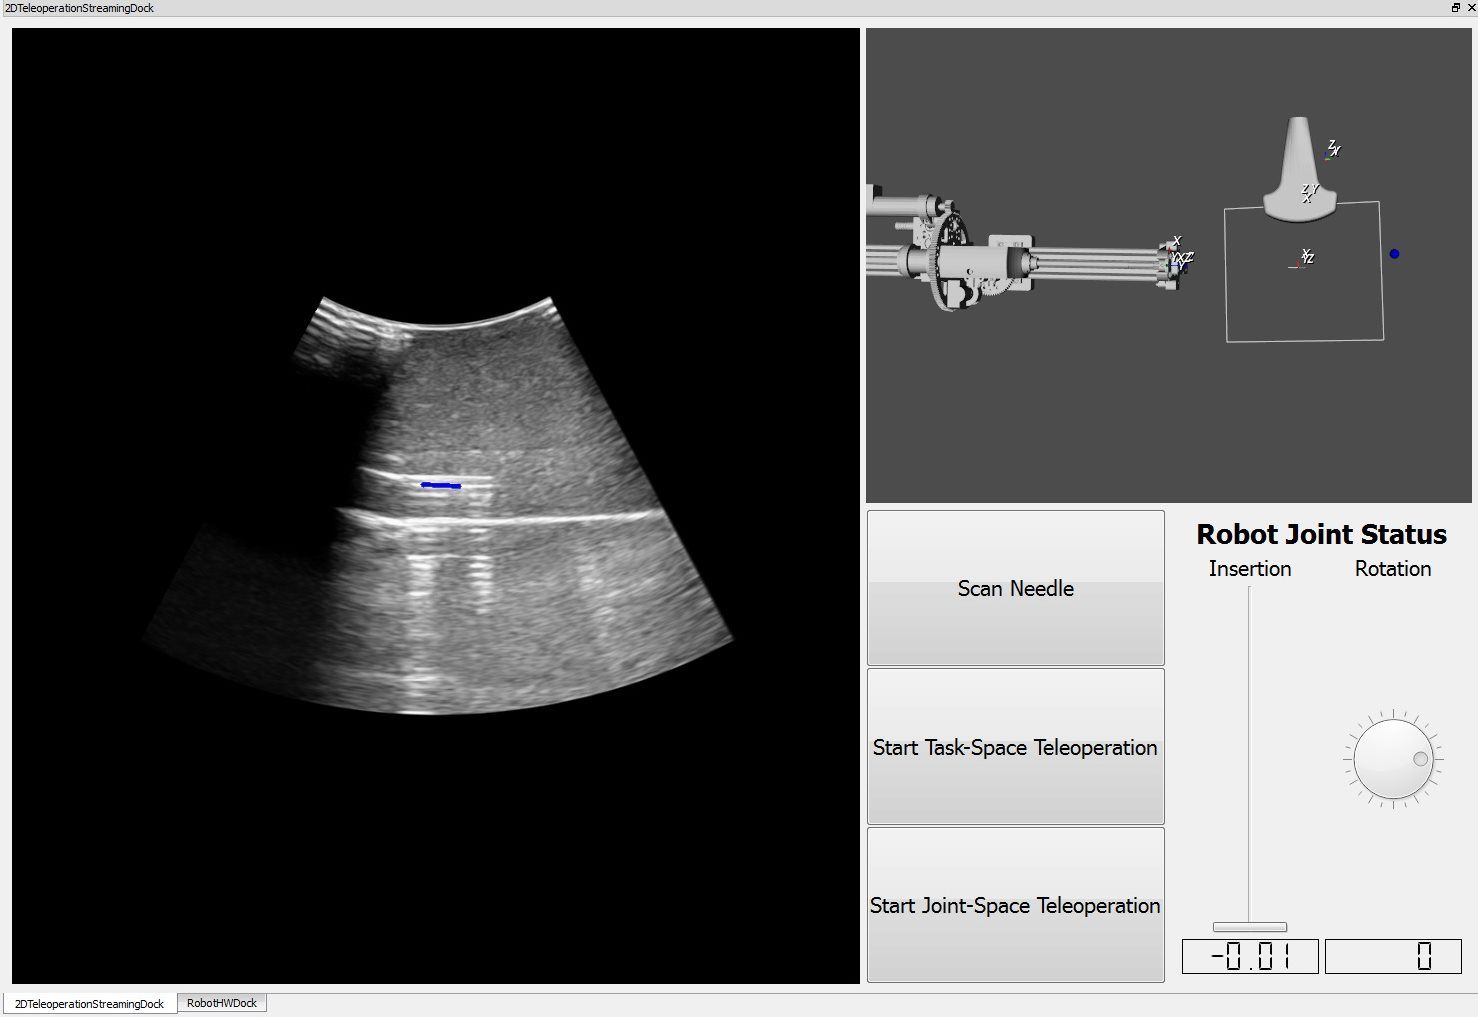
\includegraphics[width = \columnwidth]{./Images/Chapter5/GUI/GUI.jpg}%
\caption[Human-in-the-loop GUI]{Graphical user interface (GUI) for human-in-the-loop control. A screenshot shows the GUI during initial insertion, while the steerable needle tip is still within the introducer needle. Three panels are shown: (left) the live 2D ultrasound image with the current tip frame estimate over the hyperechoic needle shaft, (top right) the 3D visualization showing the ultrasound transducer pose, robot pose, tip frame estimate, and target (blue sphere), (bottom right) software control buttons and robot status readout.}
\label{fig:GUI}
\end{figure}  

\subsection{Visualization and Control Software}
A custom graphical user interface (GUI) for human-in-the-loop control was developed using Qt (Qt Company; Oslo, Norway), a cross-platform framework for application development. The GUI is shown in Fig.~\ref{fig:GUI}. The clinician user views a live 2D ultrasound image streamed from the SonixMDP console, as well as a live 3D visualization of the robot pose, transducer pose, estimate, and target. The GUI is optimized for a tablet interface. Software controls allow the user to select between the two control modes (joint-space and task-space control). The user can also set the target point $t$ by clicking in the live 2D ultrasound image. Measurements of the steerable needle tip position $p$ are similarly performed by clicking in the live 2D ultrasound image. 


%------------------------------------------------------------------------------------------
%------------------------------------------------------------------------------------------
\section{Experimental Validation}
\label{sec:HumanInTheLoopValidation}
%------------------------------------------------------------------------------------------
%------------------------------------------------------------------------------------------
\subsection{Quantification of Process and Measurement Noise}
As in Chapter 4, we first quantified process noise and measurement noise using our new robot and imaging arrangement. Process noise was again quantified by using a magnetic tracking system to precisely measure the motion of a steerable needle tip during incremental insertion along constant curvature paths. In this testing, a flexure-tip steerable needle with $l = 10$~mm and $\alpha = 45$~degrees was used. The needle was inserted along a minimum-radius-of-curvature path at a constant insertion velocity of 20 mm/s, with no rotation. The pose of the needle tip after each incremental step was compared with what was expected based on the previous pose and the process model. Although the insertion increment varied slightly due to software timing, it was generally about 0.2~mm. The needle was inserted along six paths, with 617 total measurements captured. The initial tip frame orientation was defined in the robot frame based on fixture geometry and the initial joint values $\theta$ and $l$. Radius of curvature $\rho$ for the needle was also measured using the magnetic tracking data and the least-squares fitting approach described in Chapter~3. Data analysis was performed offline using Matlab. 

Measurement noise was quantified by comparing manual tip localization results from repeated freehand 3D ultrasound scans of steerable needles in porcine liver tissue. Five repeated measurements were performed at each tip position, with 200 total measurements over five needle insertions. For each measurement, the user scanned over the needle with the ultrasound transducer, and manually selected the location of the steerable needle tip using the tablet and stylus. Data analysis was again performed offline in Matlab.

\subsection{Accuracy of Estimation Scheme}
We quantified the accuracy of our UKF estimation scheme in this application through comparison with the electromagnetic tracking system over a series of steering trials. Over four insertions in \textit{ex vivo} porcine liver, the needle was inserted while alternating between joint-space and task-space control. On each control update (synchronized to the ultrasound framerate), the calibrated electromagnetic tracker reading and UKF estimate were saved. Comparison was performed offline in Matlab.

\begin{figure}[!t]
\centering
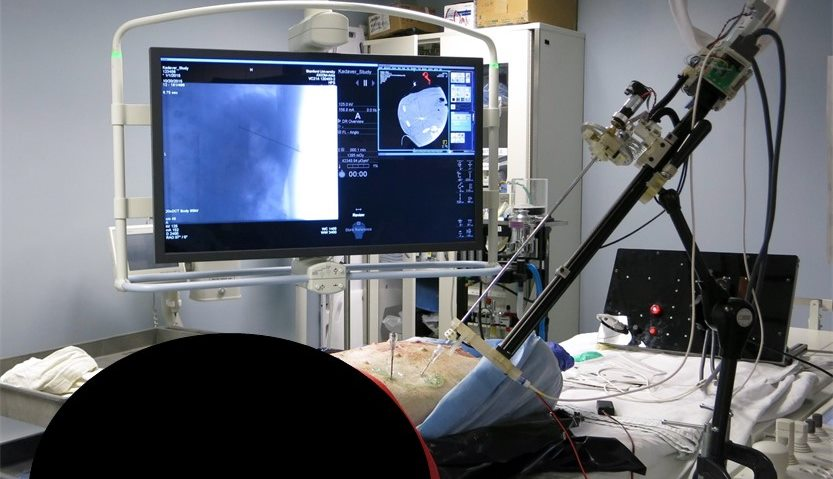
\includegraphics[width = \columnwidth]{./Images/Chapter5/CadaverSetup/CadaverSetup.jpg}%
\caption[Experimental setup for pre-clinical needle steering]{Experimental setup. The pig cadaver is mounted in supine position on the table. The needle steering robot is secured to the table rails, and connected to an introducer sheath to allow access to the liver through skin and subcutaneous fat. A second introducer sheath allows placement of target coils.}
\label{fig:CadaverSetup}
\end{figure}

\subsection{Pre-Clinical Needle Steering Experiments}
We evaluated our human-in-the-loop approach in a pre-clinical setting using an \textit{in situ} cadaveric porcine liver. Fig.~\ref{fig:CadaverSetup} shows the experimental setup for the pre-clinical needle steering experiments. A fresh pig cadaver with an undisturbed liver was obtained for testing. To prevent coagulation and preserve the mechanical properties of the liver as much as possible, heparin was administered at a dosage of 300 IU/kg prior to euthanasia. The cadaver was placed in supine position on a standard interventional radiology suite table, and was restrained to prevent tissue motion. 

\begin{figure}[!t]
\centering
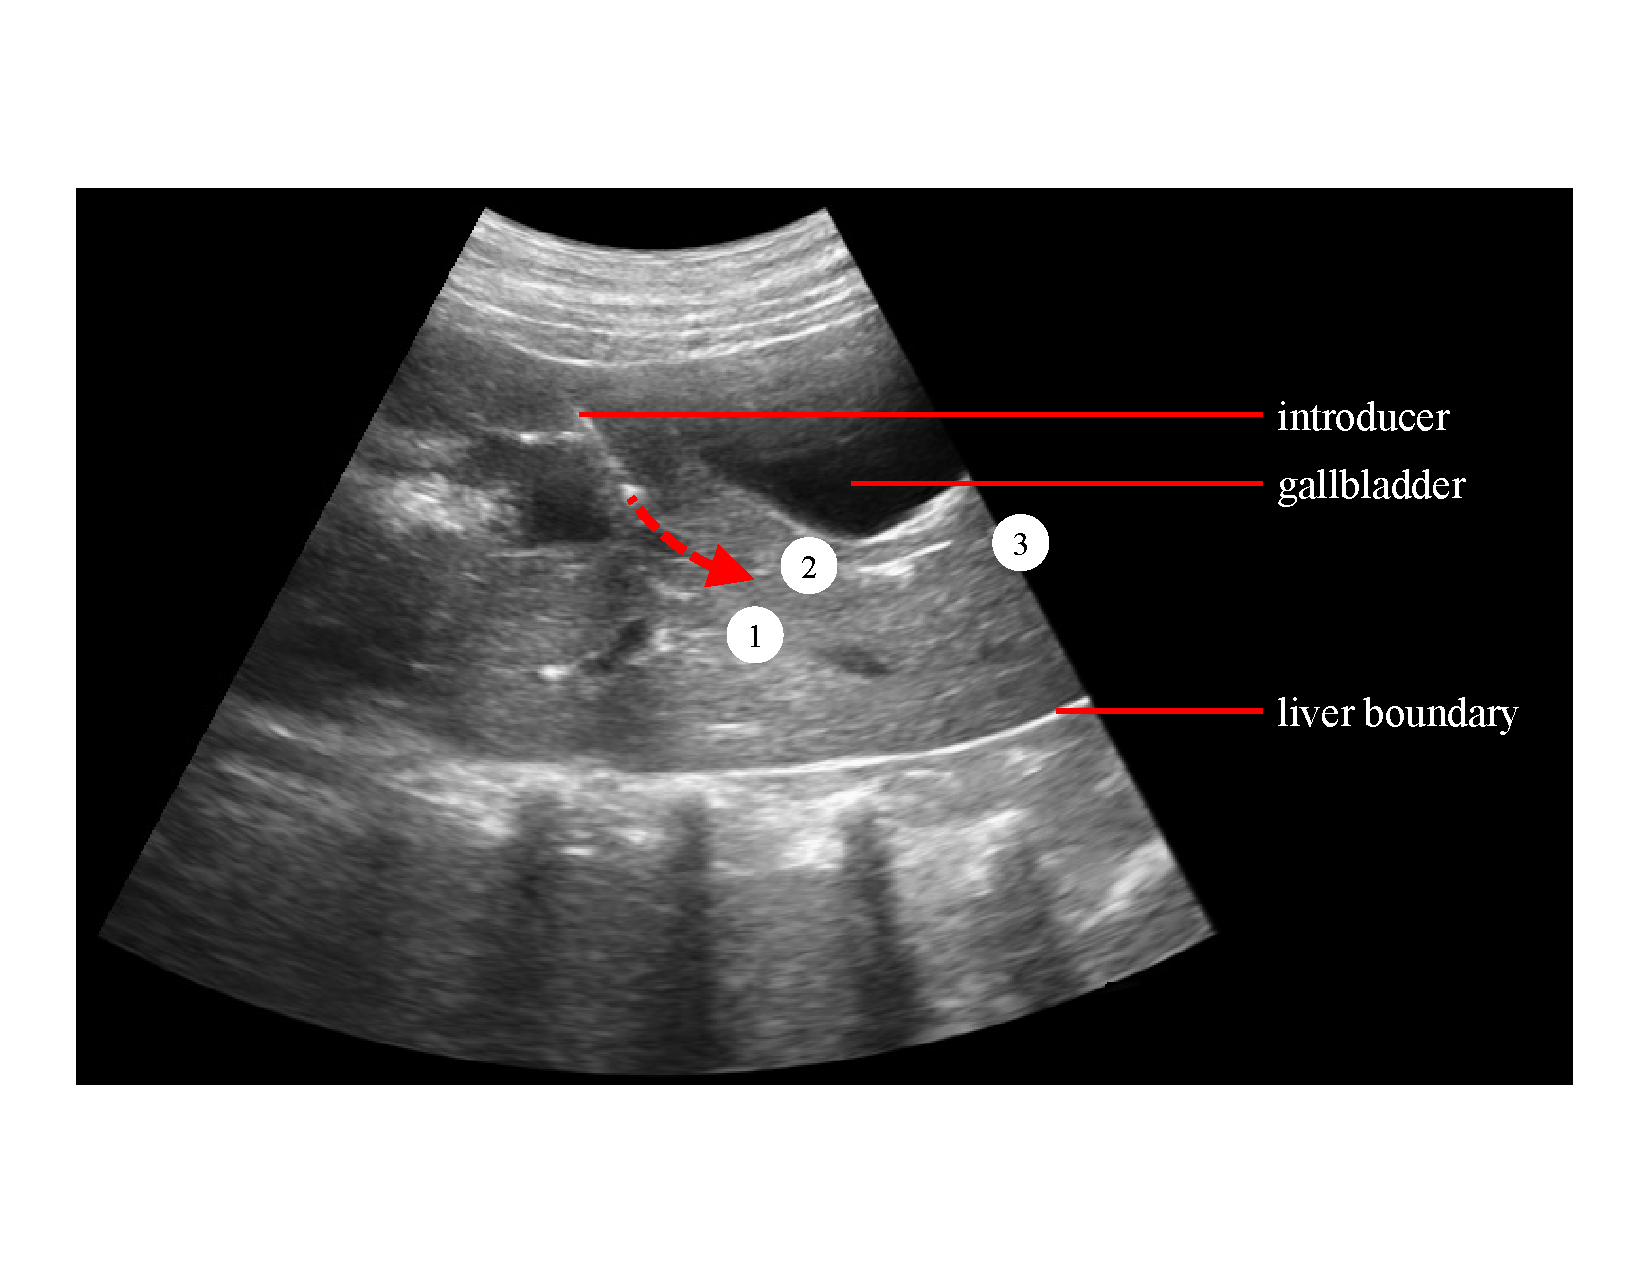
\includegraphics[width = \columnwidth]{./Images/Chapter5/CadaverTargetsUS/CadaverTargetsUS.pdf}%
\caption[Entry vector, targets and obstacles in cadaver liver]{Entry vector, targets and obstacles in cadaver liver. Three fiducials (numbered) were implanted around the gallbladder to provide targets for closed-loop needle steering. The targets were not all located within the imaging plane, and locations are approximate. The introducer needle and approximate initial path of the steerable needle are indicated, as are the gallbladder and liver boundary. }
\label{fig:CadaverTargetsUS}
\end{figure} 

After exploratory ultrasound imaging, multi-loop-coil fiducials were implanted in the liver to serve as targets. These fiducials are designed to be visible in CT imaging, but can also be visualized in ultrasound because of the gas trapped in the coils. A 15-gauge introducer needle was used to place each fiducial, and the needle was left in place during steering to aid in target identification. The three targets were increasingly difficult based on the curvature and insertion distance required to reach them from the introducer. Target 1 was located fairly close to the introducer, but required steering to avoid a section of portal vein. Target 2 was posterior to the gallbladder, and was placed by puncturing the gallbladder sack. Target 3 was also posterior to the gallbladder, but required the steerable needle to curve around the posterior aspect of the gallbladder. Fig.~\ref{fig:CadaverTargetsUS} shows the approximate locations of the three targets, projected onto the ultrasound image plane.

\begin{figure}[!t]
\centering
\includegraphics[width = \columnwidth]{./Images/Chapter5/CadaverUsers/CadaverUsers.pdf}%
\caption[User interactions during human-in-the-loop control]{User interactions during human-in-the-loop control: (a) One user manipulates the freehand 3D ultrasound transducer, scanning along the needle to localize the tip. (b) A second user interacts with the control software, selecting the location of the needle tip in an ultrasound image. }
\label{fig:CadaverUsers}
\end{figure} 

After implantation, each target was localized using the freehand 3D ultrasound and the GUI, and the needle steering robot was used to place the tip of the steerable needle at the target fiducial using task-space control. The steerable needle accessed the liver in an anterior subcostal approach, through a 15-gauge, 7-cm-long introducer needle. Steering proceeded in 10-mm increments, with a manual needle tip localization after each increment. The needle was localized using a combination of B-mode and power Doppler ultrasound; users alternated between the modes and activated vibration as needed depending on needle visibility. Typically, one user manipulated the ultrasound transducer, while a second localized the target and steerable needle in the ultrasound images. Fig.~\ref{fig:CadaverUsers} shows these interactions. In this testing, a standard mouse and monitor was used in place of the tablet interface to allow the entire team to view the images. In the future, one user could perform both the imaging and localization using the described tablet interface. Once the steerable needle reached the target depth, as measured by the output of the estimation scheme, needle insertion stopped. A DynaCT scan was then captured using an Artis Zeego imaging system (Siemens Medical Solutions, Inc.; Malvern, PA). Accuracy of tip placement was determined by measuring the distance between the tip of the steerable needle and the target fiducial in the DynaCT data.

%------------------------------------------------------------------------------------------
%------------------------------------------------------------------------------------------
\section{Results and Discussion}
\label{sec:HumanInTheLoopResults}
%------------------------------------------------------------------------------------------
%------------------------------------------------------------------------------------------
\subsection{Quantification of Process and Measurement Noise}
Across 517 samples of process noise, the mean position error (in millimeters) and mean orientation error (in degrees) were \[{\overline{p}_{w}} = \begin{bmatrix} 0.03 &-0.17 &0.01 \end{bmatrix}^{\text{T}}, {\overline{r}_{w}} = \begin{bmatrix} 0.18 &-0.03 &0.08 \end{bmatrix}^{\text{T}}.\] To find the best-fit zero-mean Gaussian distribution to the process noise, we again reflected the measured noise vectors, resulting in a sample covariance of
\begin{align*}
{\hat{Q}} = \begin{bmatrix} 
\phantom{-}0.16 & \phantom{-}0.02 	&-0.04 & -0.01 & \phantom{-}0.03 & \phantom{-}0.06\\
\phantom{-}0.02 & \phantom{-}0.16 & -0.02 & -0.05 & \phantom{-}0.03 & \phantom{-}0.01 \\ 
-0.04 & -0.02 & \phantom{-}0.46 & -0.10 & \phantom{-}0.01 & -0.03 \\
-0.01 & -0.05 & -0.10 & \phantom{-}0.24 & \phantom{-}0.01 & \phantom{-}0.02 \\
\phantom{-}0.03 & \phantom{-}0.03 & \phantom{-}0.01 & \phantom{-}0.01 & \phantom{-}0.05 & \phantom{-}0.03 \\
\phantom{-}0.06 & -0.01 & -0.03 & \phantom{-}0.04 & \phantom{-}0.03 & \phantom{-}0.24\\ 
\end{bmatrix}.
\end{align*}

In the measurement noise experiment, we again assumed the mean of repeated localization at each tip pose was the true needle pose. Across 200 total measurements, the sample covariance (of the position components only) was 
\begin{align*}
{\hat{R}} = \begin{bmatrix} 
\phantom{-}2.29 & \phantom{-}1.58 & \phantom{-}2.51 \\ 
\phantom{-}1.58 & \phantom{-}6.97 & \phantom{-}2.19 \\ 
\phantom{-}2.51 & \phantom{-}2.19 & \phantom{-}11.4 \\ 
\end{bmatrix}.
\end{align*}

\begin{figure}[!t]
\centering
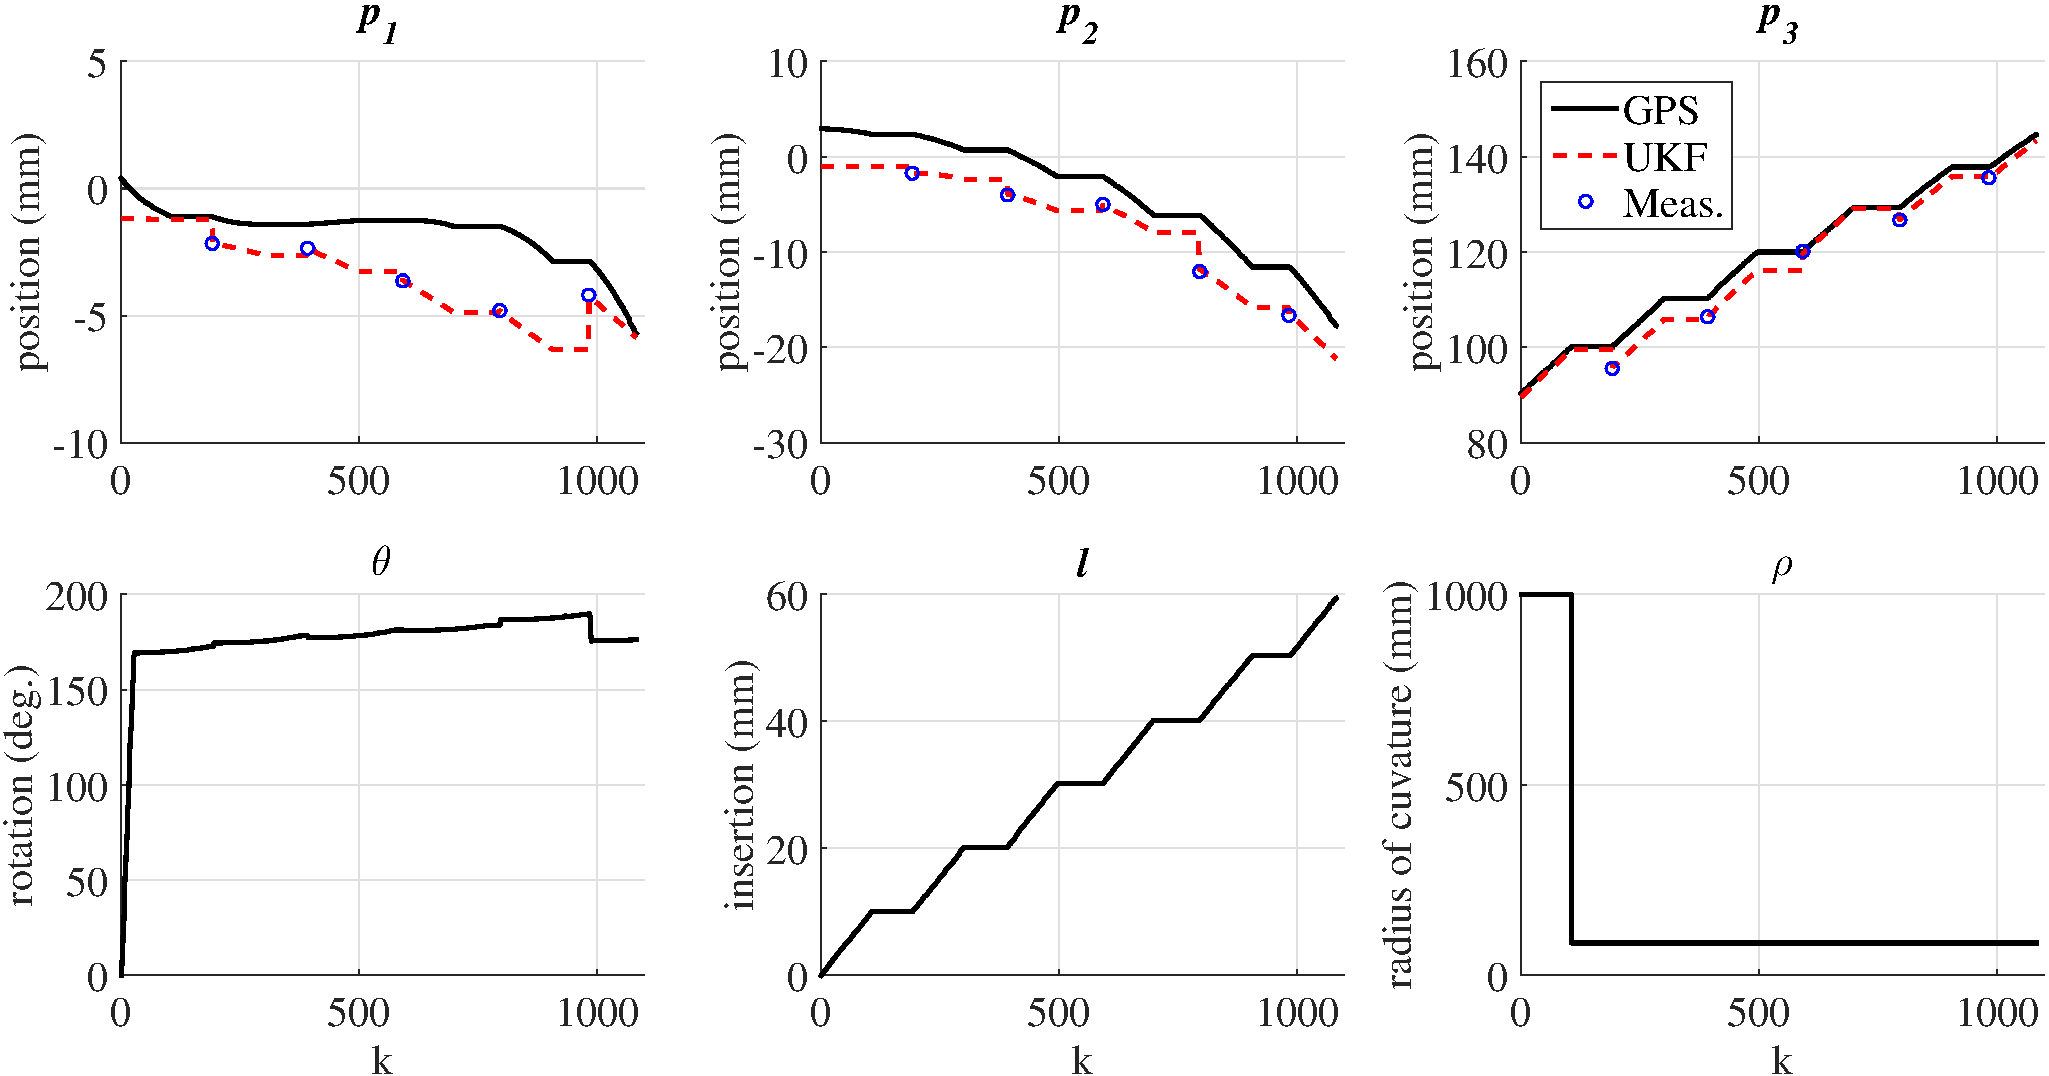
\includegraphics[width = \columnwidth]{./Images/Chapter5/UKFAccuracy/UKFAccuracy.pdf}%
\caption[UKF accuracy results]{UKF estimation scheme accuracy results. Comparison of calibrated and filtered electromagnetic tracker position (GPS) with estimated position (UKF). Measurements are also indicated. Robot joint variables ($\theta$, $l$) and radius of curvature $\rho$ are also shown. For UKF updates, $\rho$ is set to 1000~mm while the needle is inside the introducer sheath. }
\label{fig:UKFAccuracy}
\end{figure}  

\subsection{Accuracy of Estimation Scheme}
Across 5199 data points from four separate insertions, the mean distance between the estimated position and the electromagnetic tracker measurement was 4.6~mm. Fig.~\ref{fig:UKFAccuracy} shows a comparison of the UKF estimate and the electromagnetic tracking system, along with system inputs. Estimation error was generally largest in the robot frame's $y$-axis direction. In these tests, this corresponded to mismatches in the needle radius of curvature $\rho$. The UKF estimation scheme assumed a constant $\rho =$~85~mm once the steerable needle left the introducer needle. This value of $\rho$ was based on initial measurements over complete insertions in the liver tissue sample. 

Several practical issues limit the use of the electromagnetic tracker inside the needle tip as a gold standard. First, the tracker is sensitive to electromagnetic noise from the vibration motor during actual steering. Second, the vendor-supplied calibration of the tracked ultrasound transducer is not perfectly accurate. Finally, it is impossible to place the electromagnetic transducer right at the needle tip (because of the rigid bent-tip section), so a tip calibration must be applied to the raw tracking data. This tip calibration introduces additional tracking error.

\subsection{Pre-Clinical Needle Steering Experiments}
Fig.~\ref{fig:CadaverDoppler} shows examples of in-plane and transverse power Doppler images of the vibrating needle in the \textit{in situ} cadaveric porcine liver. The disposable vibration device was able to generate a recognizable Doppler signature along the shaft of the needle in a realistic pre-clinical imaging arrangement. The Doppler response tended to be more irregular and less localized during the initial insertion, especially while the steerable needle tip was still in the introducer needle. As seen in Fig.~\ref{fig:CadaverDoppler}(a), the image analysis methods presented in Chapter 2 would likely not have been able to generate a useful measurement of the tip pose. Once the steerable needle was inserted farther into the tissue, the Doppler response became more regular and localized around the steerable needle, as seen in Fig.~\ref{fig:CadaverDoppler}(b). 

\begin{figure}[!t]
\centering
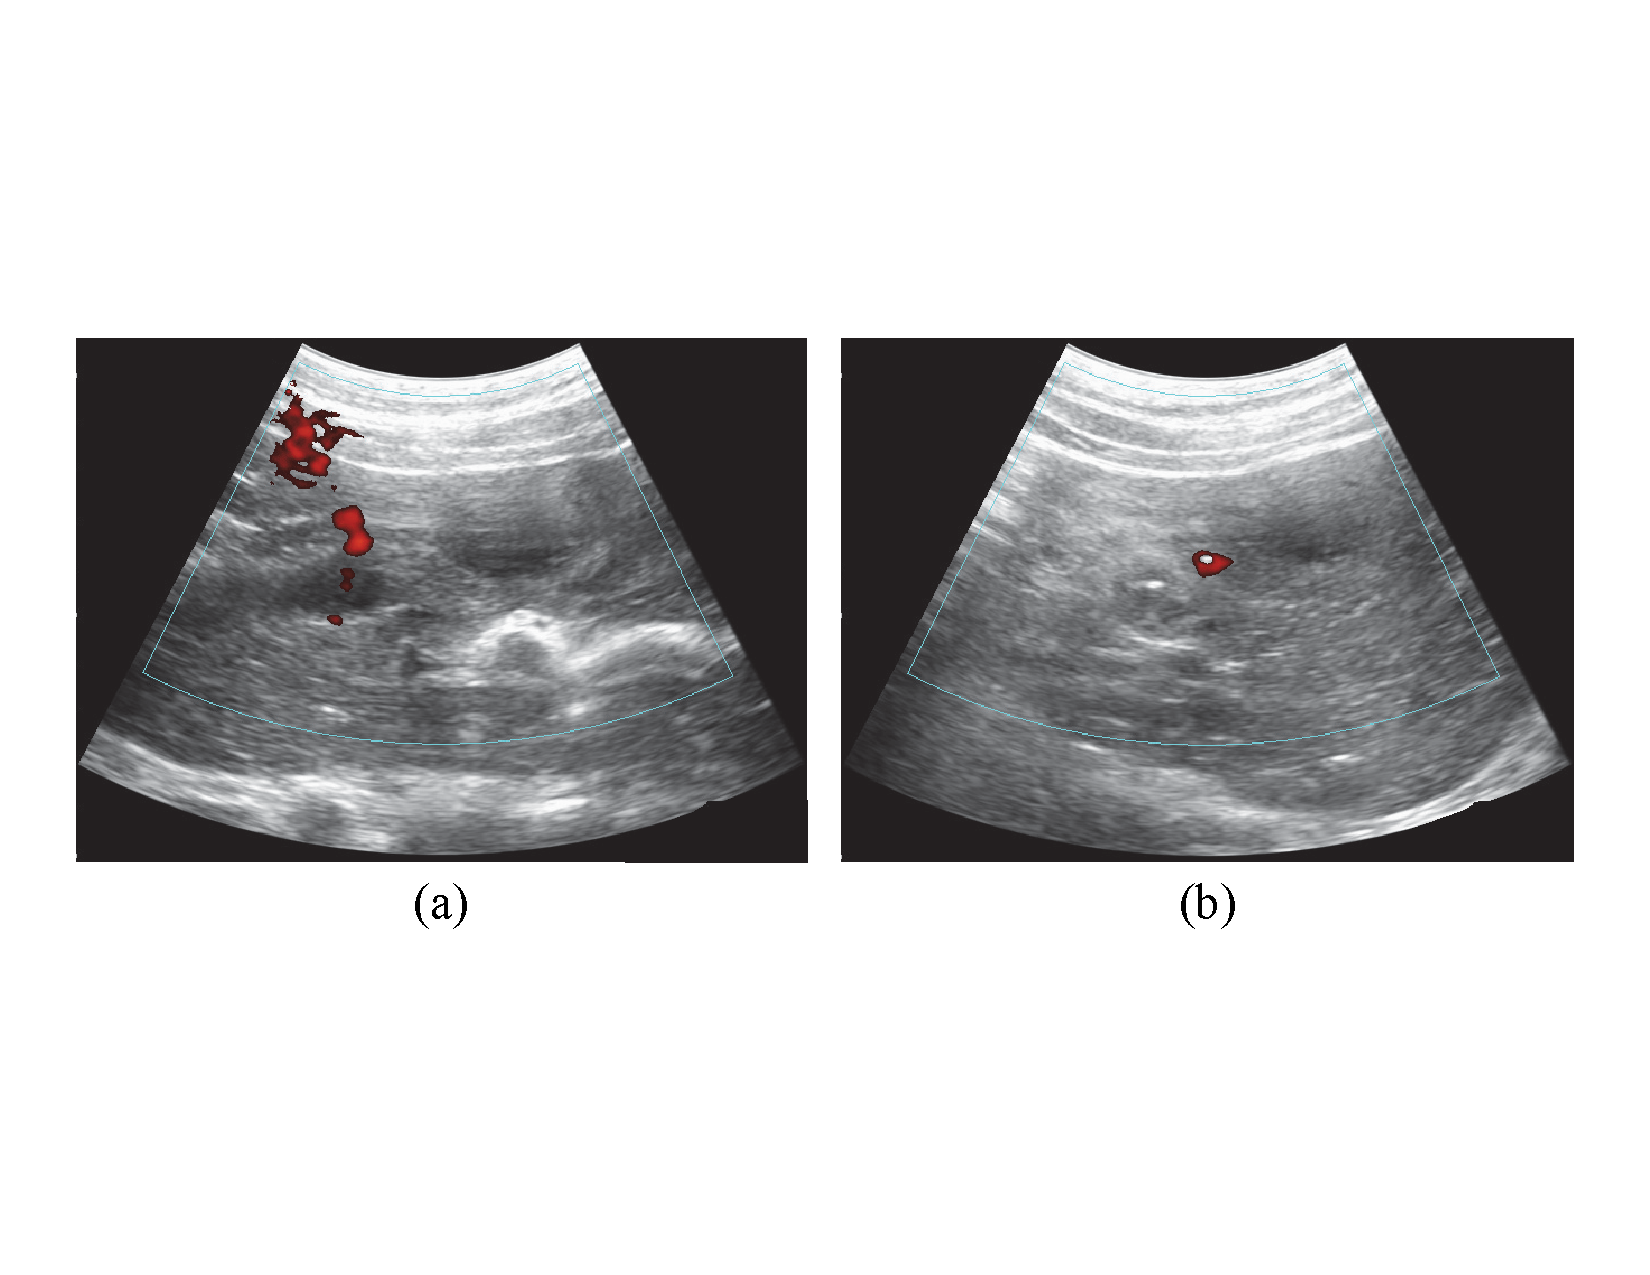
\includegraphics[width = \columnwidth]{./Images/Chapter5/CadaverDoppler/CadaverDoppler.pdf}%
\caption[Power Doppler ultrasound images of steerable needle in pig cadaver]{Power Doppler ultrasound images of steerable needle in pig cadaver: (a) an in-plane image of the introducer needle and steerable needle. (b) A transverse image of the steerable needle.  }
\label{fig:CadaverDoppler}
\end{figure}  

Table~\ref{table:CadaverTargets} lists target positions and tip placement error for the three targets. For Target 1, the final tip placement error measured in DynaCT was 4.24~mm, which approaches the level of accuracy required in ablation of liver tumors~\cite{Crocetti2008}. This target required less deviation from the initial insertion vector than Target 2 and Target 3. Fig.~\ref{fig:CadaverAtTarget} shows the software interface at the completion of steering to Target 1. 

\begin{table}[!t]
% increase table row spacing, adjust to taste
\renewcommand{\arraystretch}{1.3}
\centering
\caption{Targets and errors in pre-clinical needle steering experiments}
\label{table:CadaverTargets}
\begin{tabulary}{\columnwidth}{| C | C | C | C | C | C | C | }
\hline
Target & $t_x$ (mm) & $t_y$ (mm) & $t_z$ (mm) & $e_{\text{final}}$ (mm) \\
\hline
1 & -4.1 & -7.1 & 191.5 & 4.24 \\
\hline
2 & 12.4 & -6.8 & 217.0 & 21.4 \\
\hline
3 & 28.7 & -4.6 & 189.8 & 21.6 \\
\hline
\end{tabulary}
\end{table}

For Target 2, the intermediate target placed posterior to the gallbladder by puncturing the gallbladder sack, the tip placement error measured in DynaCT was 21.4~mm. This target required a larger deviation from the initial insertion vector than Target 1, and the tip placement error was correspondingly larger. The large error appeared to be a result of insufficient curvature, rather than controller error. In other words, the estimation and control software kept the needle curving towards the target throughout insertion, but the needle simply did not curve strongly enough to reach the target.

Target 3, the difficult target placed around the posterior aspect of the gallbladder, required the largest deviation from the original insertion vector. For Target 3, the tip placement error measured in DynaCT was 21.6~mm. As with Target 2, this again appeared to be a result of insufficient curvature. Fig.~\ref{fig:CadaverTargetsCT} shows DynaCT images captured after steering to each of the three targets. 

Fig~\ref{fig:FailedCadaverTargetsCT} shows an example of an additional steering trial that was halted. In this trial, we attempted to steer to the tip of an introducer needle located near Target~3, without implanting a fiducial. In this trial, the needle tip became stuck about halfway to the target, and the shaft of the needle buckled. This buckling behavior would be undesirable in a pre-clinical setting.

\begin{figure}[!t]
\centering
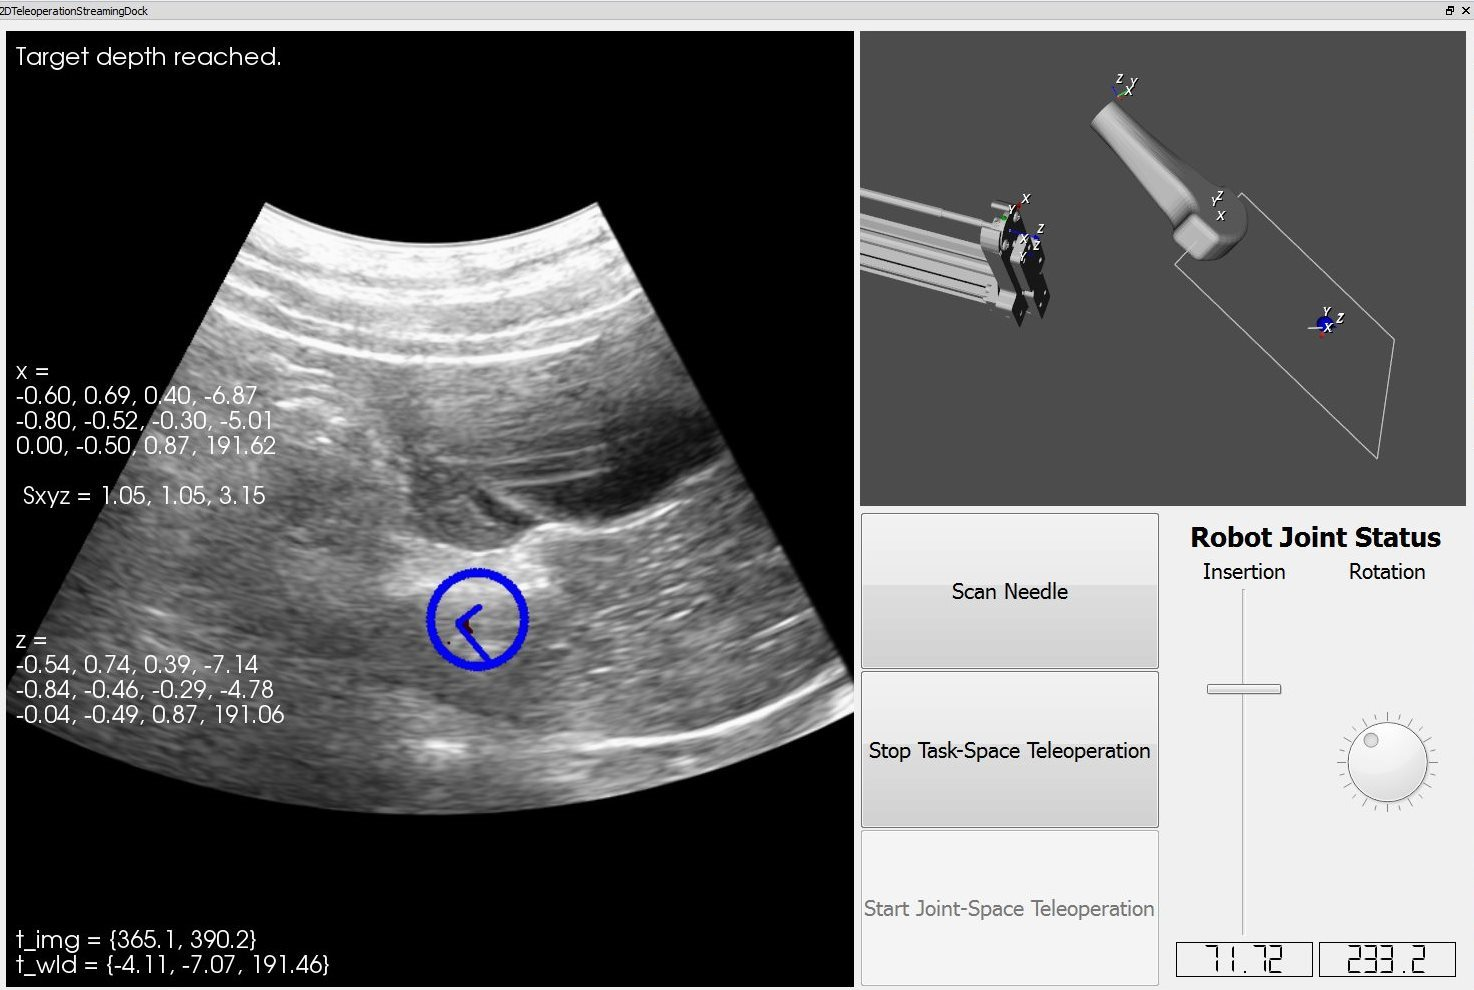
\includegraphics[width = \columnwidth]{./Images/Chapter5/CadaverAtTarget/CadaverAtTarget.jpg}%
\caption[GUI at completion of pre-clinical experiment]{View of GUI at completion of pre-clinical experiment with Target 1. The estimated position (blue lines) is shown within the target icon (blue circle) in the live ultrasound image. A small Doppler response is seen at the needle tip. The target was located posterior to the gallbladder.}
\label{fig:CadaverAtTarget}
\end{figure}  

\begin{figure}[!t]
\centering
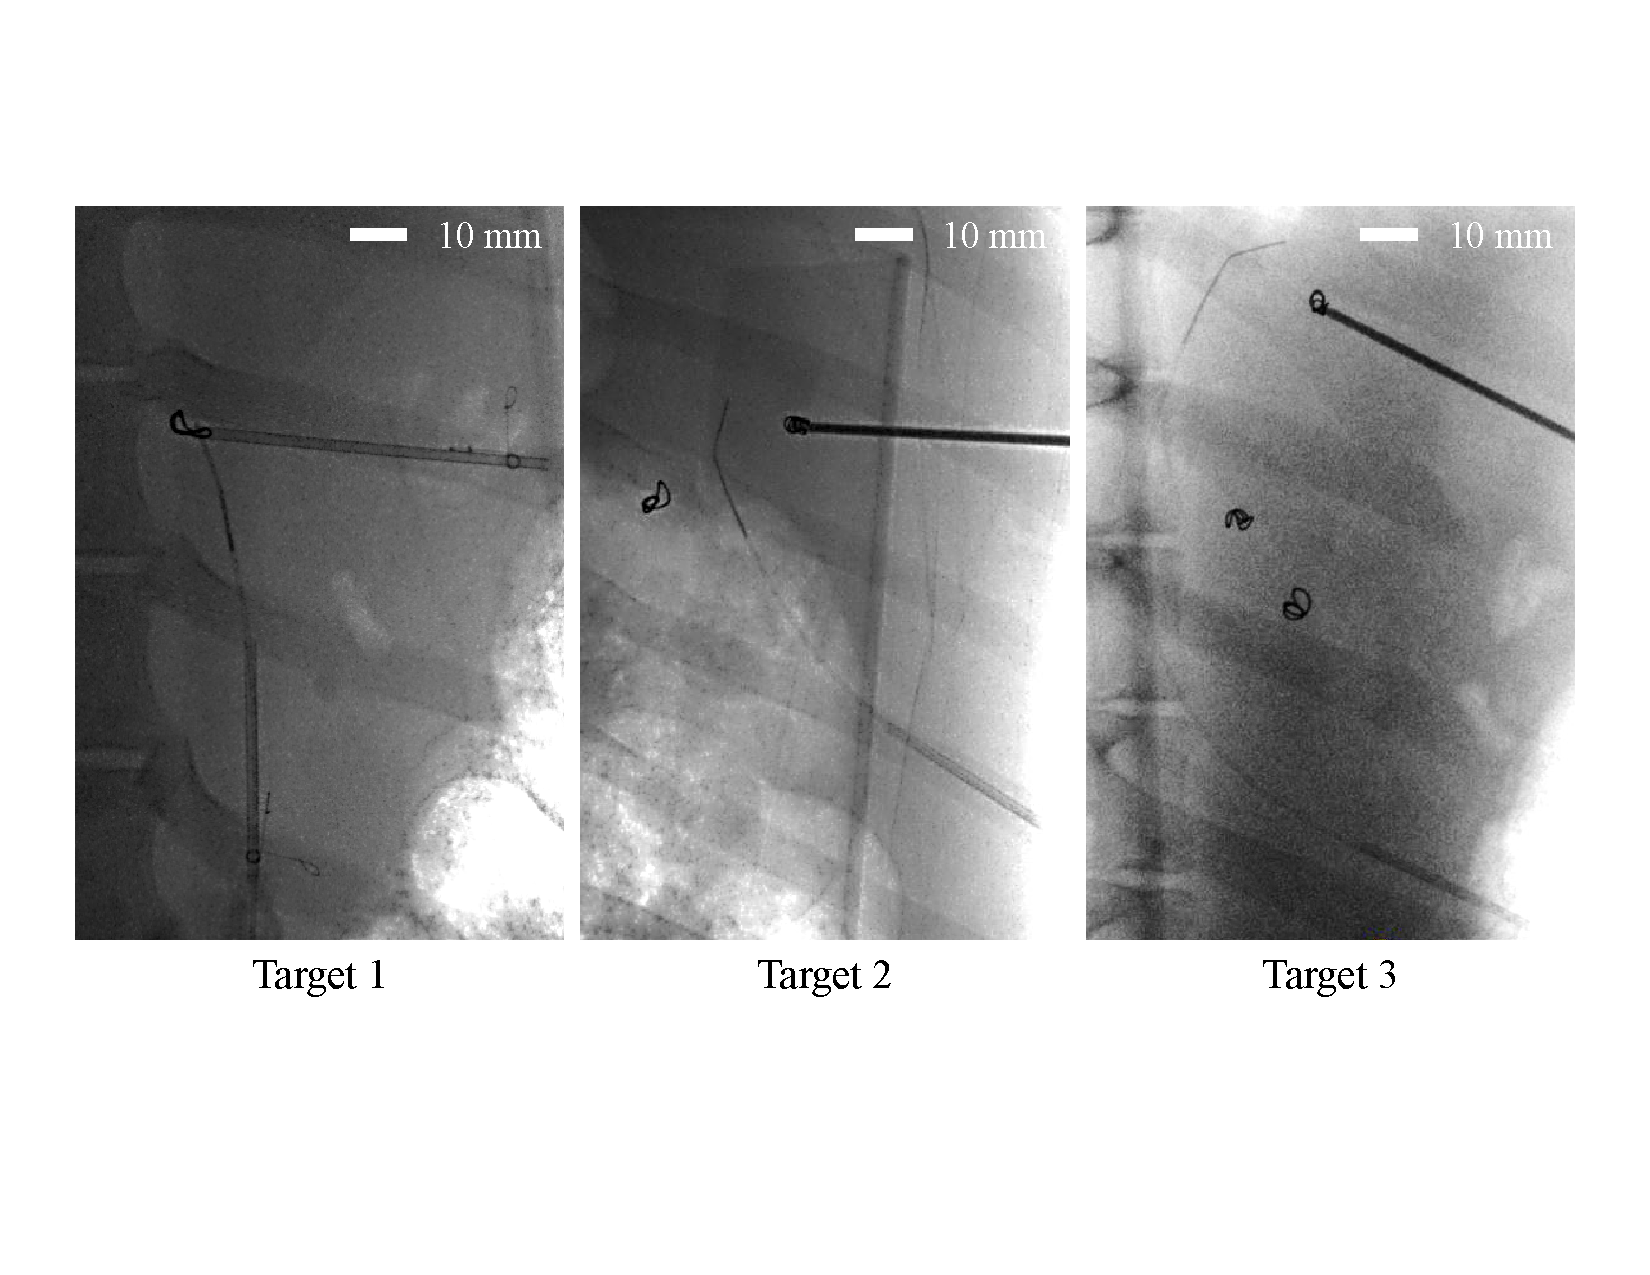
\includegraphics[width = \columnwidth]{./Images/Chapter5/TargetsCT/TargetsCT.pdf}%
\caption[DynaCT images captured after pre-clinical experiments]{DynaCT images captured after completion of pre-clinical needle steering experiments in porcine cadaver. Each image depicts the introducer needle, steerable needle, and target fiducial with the second introducer used for implantation.}
\label{fig:CadaverTargetsCT}
\end{figure} 

\subsection{Discussion}
All three targets placed in the pre-clinical experiment were theoretically reachable from the introducer with $\rho =$~50~mm. Based on the results of the bench-top curvature tests described in Chapter~3, we expected the steerable needles used in this experiment to achieve $\rho =$~50~mm; however, the curvature was worse in the \textit{in situ} cadaveric liver than in the excised liver samples. As a result, the steerable needles did not curve strongly enough to reach Target~2 or Target~3. The most likely explanation is the mechanical differences between a complete liver and a liver sample. For example, the needle's path through the \textit{in situ} liver may have crossed connective tissues or lobe boundaries that the smaller excised samples did not contain. Also, the \textit{in situ} liver was constrained differently around its boundary than the bench-top samples. Several other complicating factors may also have affected curvature. The introducer needle was displaced perpendicular to the needle axis after connecting it to the needle steering robot. The tension in the surrounding tissue may have applied additional force to the needle tip as it exited the introducer inside the liver. Also, ultrasound imaging of the \textit{in situ} liver required a larger contact force between the ultrasound transducer and the cadaver skin than in bench-top testing, resulting in displacement of the liver on the order of centimeters. Overall, the performance difference between bench-top and pre-clinical testing emphasizes the importance of testing in more realistic clinical environments, and the need to improve needle curvature even further. Suggestions for this are discussed in the next chapter.

\begin{figure}[!t]
\centering
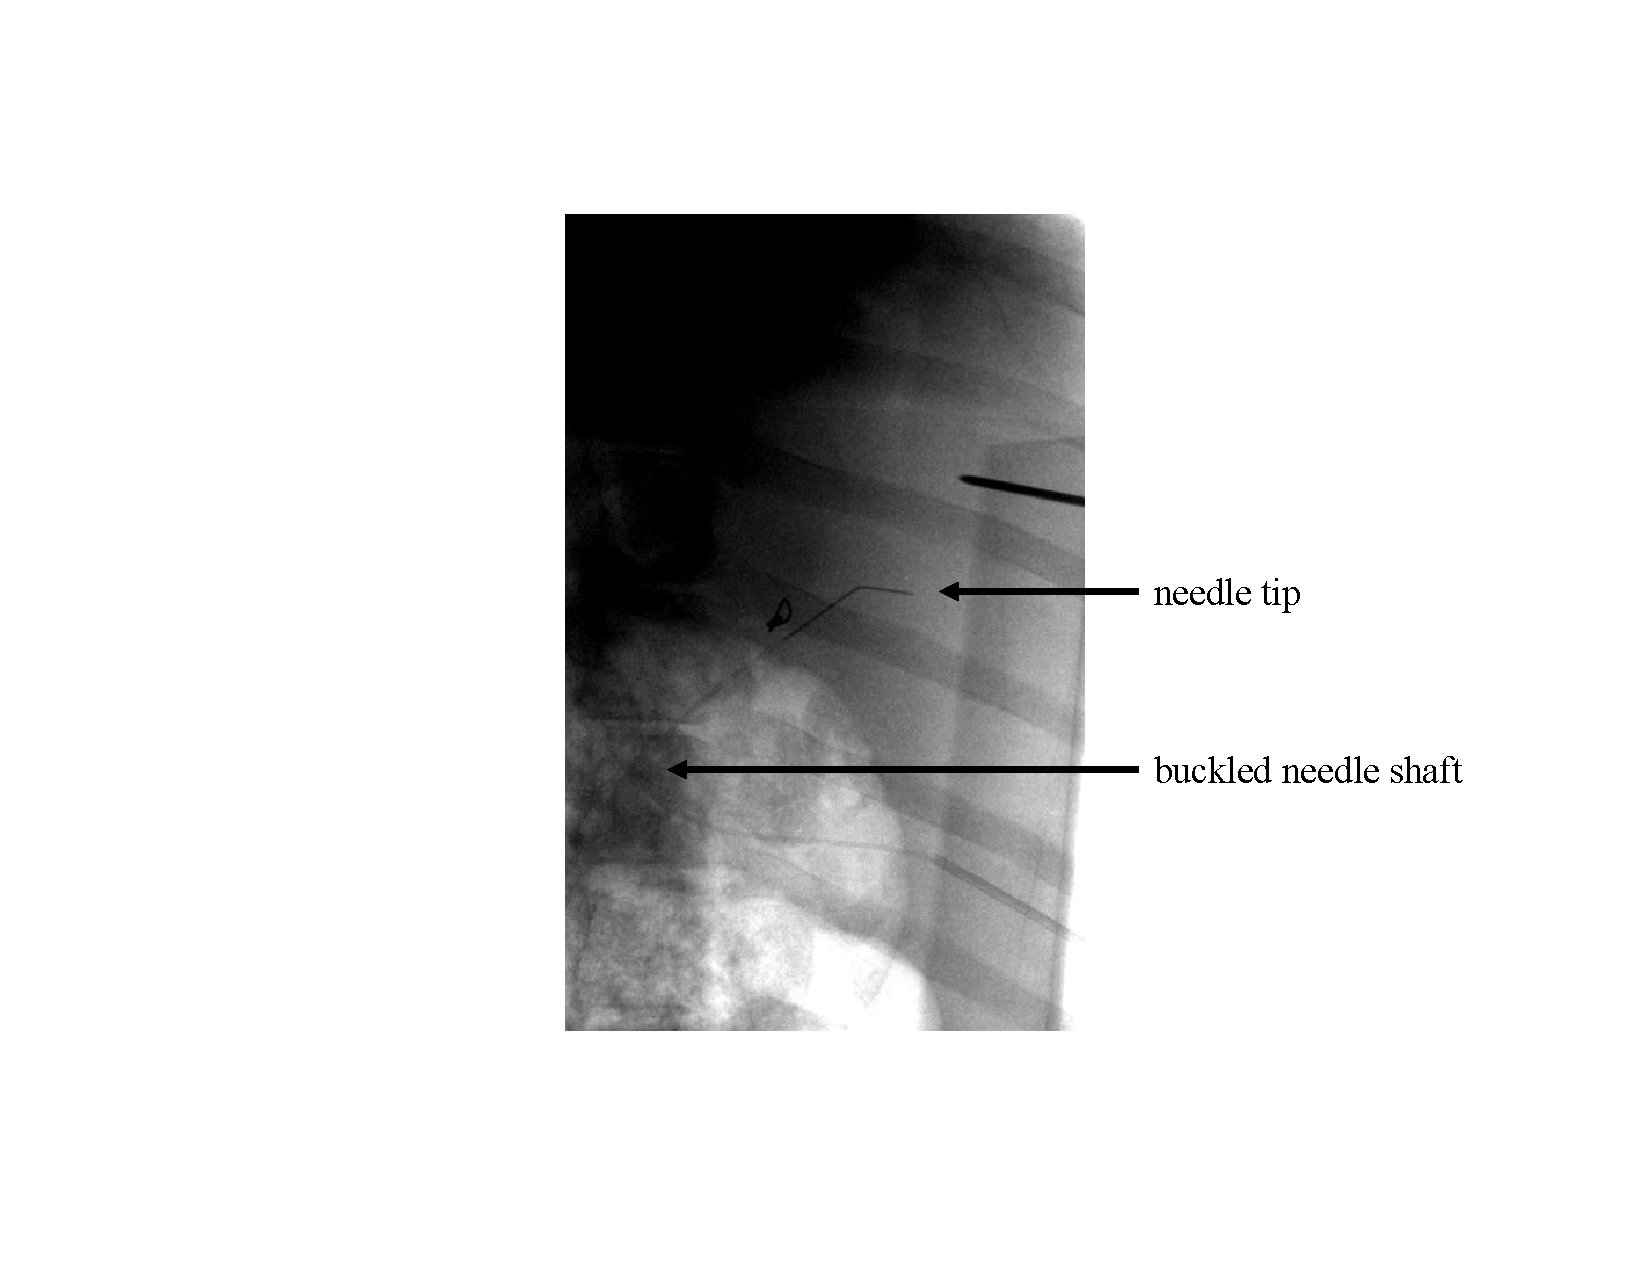
\includegraphics[width = \columnwidth]{./Images/Chapter5/TargetsCT/FailedTargetsCT.pdf}%
\caption[DynaCT images captured after failed pre-clinical experiment]{DynaCT image captured after completion of pre-clinical needle steering experiment in porcine cadaver. The image depicts the introducer needle, steerable needle, and target fiducial with the second introducer used for implantation. In this case, needle tip stuck, causing buckling of the needle shaft.}
\label{fig:FailedCadaverTargetsCT}
\end{figure} 

Several important problems remain to be solved before our methods would be successful in a live-animal experiment. First, the cutting behavior of bent-tip steerable needles in liver must be improved. Although our system was able to place the steerable needle tip at the three targets described in this chapter with varying levels of accuracy, the needle tip also occasionally became stuck, occasionally causing severe buckling of the needle shaft. DynaCT images of the stuck needle tip showed no obvious impeding structure. In other words, the needle tip was not able to consistently cut through ordinary liver parenchyma. This mechanical catching might be greatly reduced by producing steerable needles with sharper tips. In the current implementation, the Nitinol flexure tip was sharpened using a grinding wheel, but the resulting edge was not nearly as sharp as a clinical trocar or introducer needle.

A second important problem is the management of respiratory motion. In the cadaver experiment described in this chapter, we elected not to ventilate the cadaver to simulate respiratory motion. In a live-animal experiment or clinical application, such motion is unavoidable. One strategy might be to gate control of the needle motion to the respiratory cycle. Alternatively, high-frequency jet ventilation~\cite{Denys2014} might be used to minimize respiratory motion.

A final important problem is the selection and placement of targets for the needle steering experiments. It was remarkably difficult to place the introducer needle and fiducial markers to provide a realistic but feasible target geometry for each trial. Relative motion of the introducer needles during connection of the robot, and displacement of the needles during penetration of the tough skin and subcutaneous fat were the main difficulties. Although it might be possible to use natural anatomical targets such as vessel branches, it is generally difficult to resolve these structures accurately based on DynaCT data because of limited soft-tissue contrast.

\subsubsection{Summary}
In this chapter we have presented a pre-clinical system for ultrasound-guided needle steering. To our knowledge, the experiments we have described are the first example of closed-loop image-guided needle steering in an animal model. While important challenges remain, particularly improving the steering behavior and minimum radius of curvature of bent-tip needles in liver tissue, the methods described in this chapter should enable further pre-clinical testing in live animals to proceed in short order.  

